\chapter{Prototipna implementacija}
Radi praktične demonstracije funkcionalnosti generativnih suparničkih mreža, implementirali smo varijantu modela temeljenu na progresivnom rastu \citep{karras2017progressive}. U ovom poglavlju, predstavit ćemo detaljno korištenu arhitekturu uz pojašnjenje specifičnosti karakterističnih upravo za ovaj tip modela. Predstavit ćemo i skup podataka na kojemu smo trenirali te dobivene rezultate.

\section{Arhitektura}
Kao što smo već ranije spomenuli, osnovna ideja kod progresivnog rasta generativnih suparničkih mreža jest slijedno treniranje na inačicama ulaznog skupa podataka rastućih rezolucija. Primjerice, početni model istreniramo na skupu slika rezolucije $4 \times 4$. Nakon što postupak optimizacije konvergira, model nadogradimo i povećamo rezoluciju na $8 \times 8$ i nastavimo s treniranjem te ovakav postupak ponavljamo dok ne postignemo željenu rezoluciju.

Da bismo pojasnili na koji način je ovaj princip učenja implementiran, pogledajmo prvo osnovnu građevnu jedinicu našeg modela: blok. Naravno, blokovi za diskriminator (slika \ref{disc_blocks}) i generator (slika \ref{gen_blocks}) se ponešto razlikuju, ali im je funkcionalnost slična. 

\begin{figure}[h]
\centering
		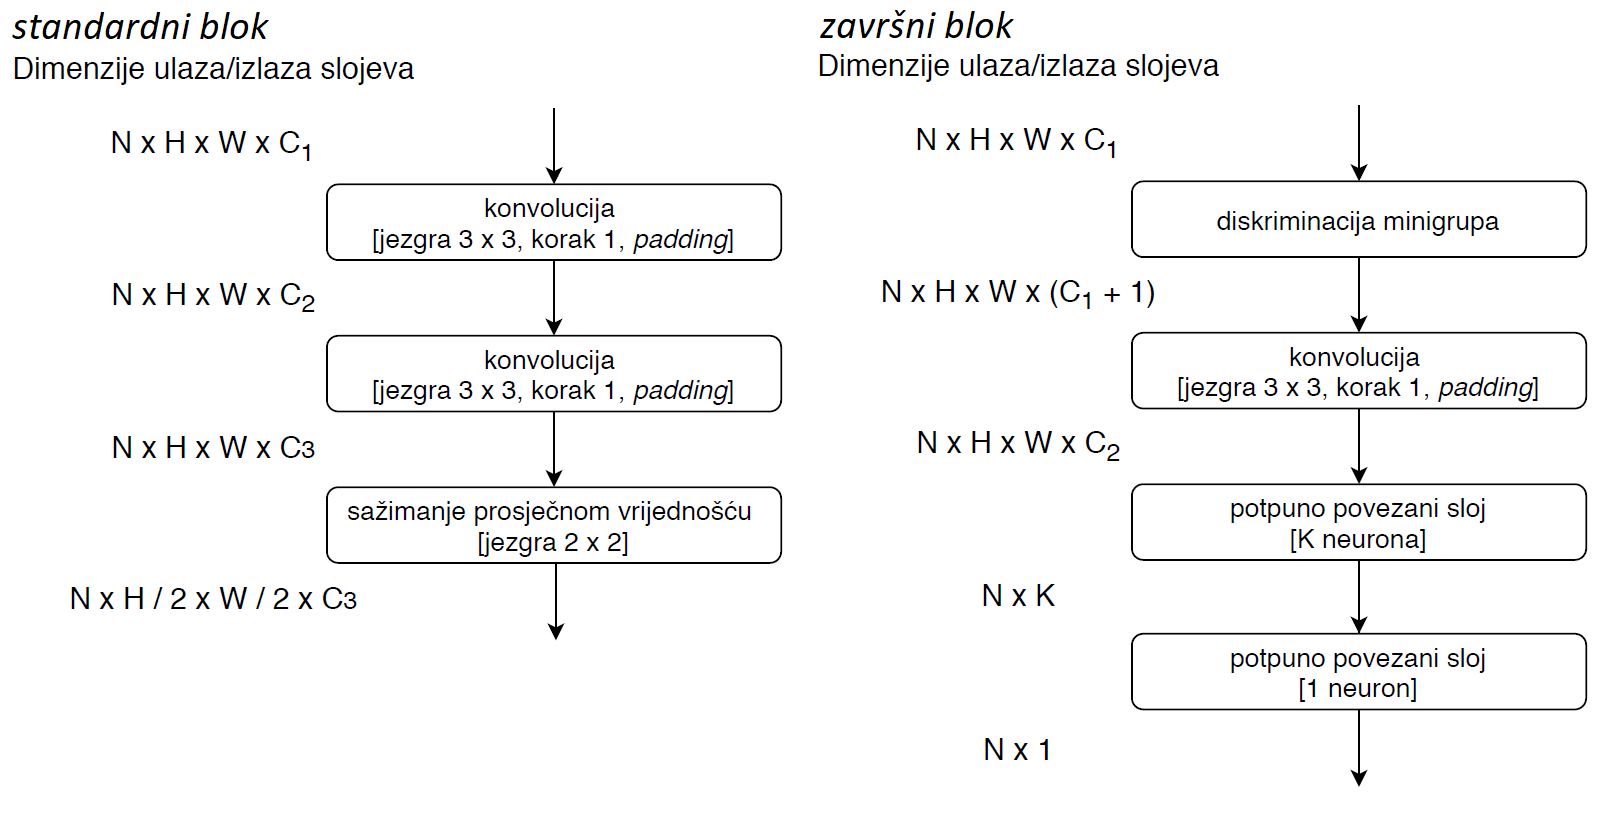
\includegraphics[height=0.5\textwidth]{images/blokovi_diskriminatora.png}
\caption{Shema korištenih blokova u diskriminatoru}
\label{disc_blocks}
\end{figure}

\begin{figure}[h]
\centering
		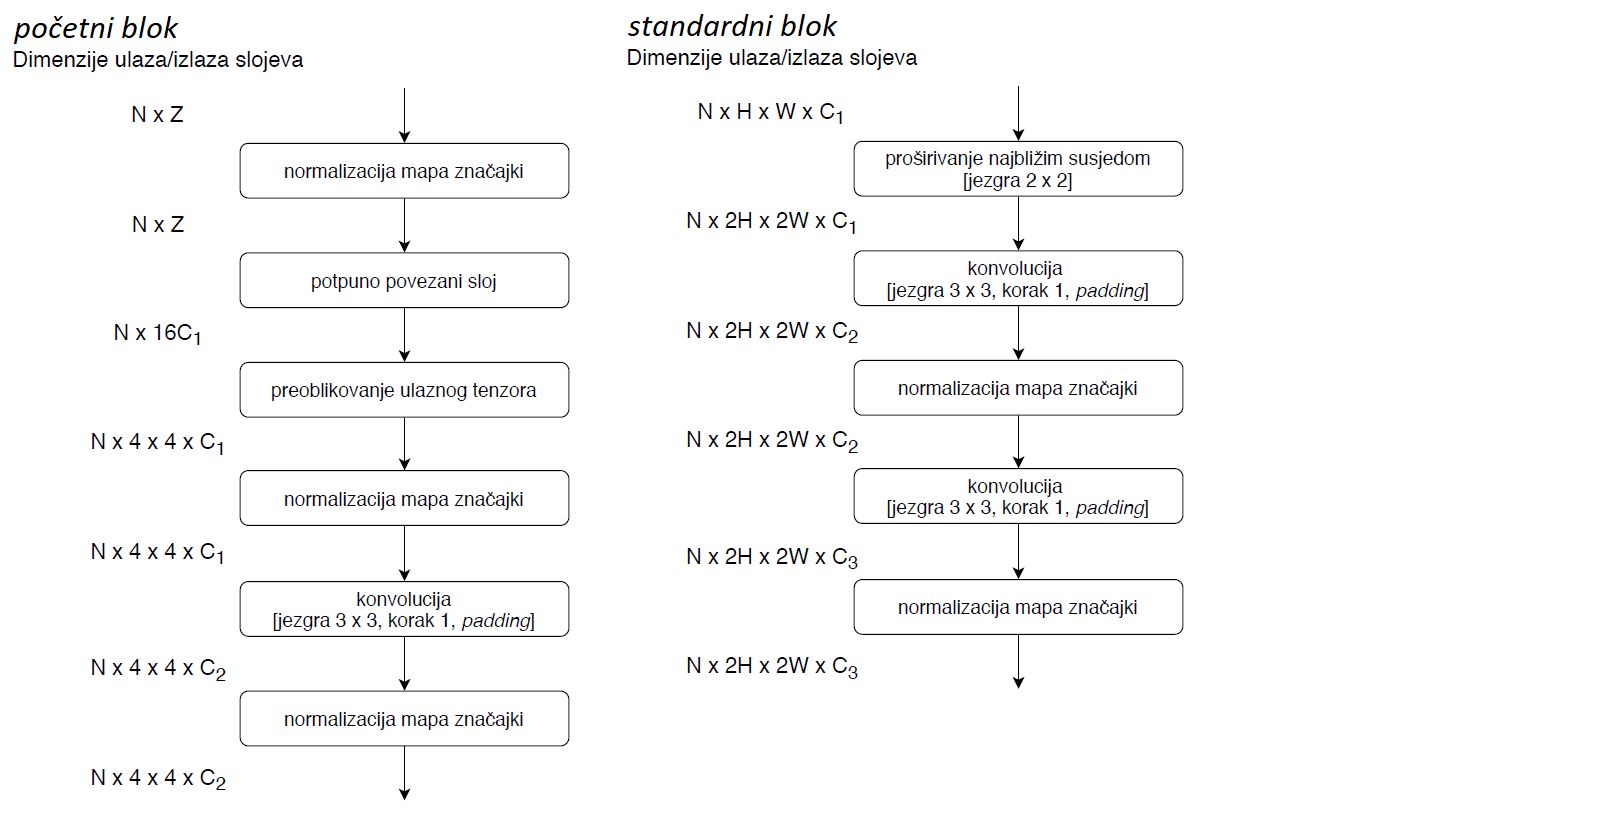
\includegraphics[height=0.7\textwidth]{images/blokovi_generatora.png}
\caption{Shema korištenih blokova u generatoru}
\label{gen_blocks}
\end{figure}

Zadaća jednog bloka jest povećati ili smanjiti rezoluciju ulaznog tenzora (ovisno radi li se o diskriminatoru ili generatoru) te ekstrahirati važne značajke dobivenog rezultata. Nadogradnja modela tada se svodi na eliminaciju izlaznog sloja te dodavanje bloka i novog izlaznog sloja na kraj (u slučaju generatora) ili eliminaciju ulaznog sloja te dodavanje bloka i novog ulaznog sloja (u slučaju diskriminatora). Ovakav pristup možemo promatrati kao tehniku nadziranog predtreniranja \citep{cupic2019nadpred} prilagođen našem zadatku. Napomenimo još da težine nižih blokova nisu "zamrznute" za vrijeme treniranja na višim rezolucijama, nego ih i dalje optimiramo pomoću gradijentnog spusta.

Osim navedenih blokova, koristimo i konvolucijske slojeve čija je zadaća osigurati tranziciju tenzora iz prostora slika (tenzora oblika $D \times D \times C$, gdje je $D$ duljina stranice slike, a $C$ broj kanala) u prostor mapa značajki, odnosno tenzora oblika $D \times D \times F$, gdje je $F$ broj mapa značajki. Razlika je što kanali predstavljaju informacije potrebne za vizualizaciju slike, dok mape značajki modeliraju i informacije o strukturi pohranjene na slikama. Ovi konvolucijski slojevi koriste se kao ulazni sloj u diskriminatoru te izlazni sloj u generatoru.

Broj mapa značajki i kod različitih rezolucija se razlikuje. Kako autori u radu ne navode kako ih određuju, za odabir broja mapa značajki koristimo prilagođenu funkciju koja se može pronaći na \citep{progressive_gan_git}.

U svim se slojevima kao aktivacijska funkcija koristi propusna zglobnica \engl{Leaky ReLU}, osim izlaznim slojevima generatora i diskriminatora gdje je aktivacijska funkcija linearna. Propusna je zglobnica definirana kao:
\begin{equation*}
f(x; \alpha) = 
	\begin{cases}
		x, \quad \text{ako } x > 0,\\
		\alpha x, \quad \text{inače} 
	\end{cases}
\end{equation*}
$\alpha$ je uobičajeno mali pozitivan broj, u našem slučaju 0.2. Popularna aktivacijska funkcija zglobnica \engl{ReLU} je specijalni slučaj propusne zglobnice gdje je $\alpha = 0$.

Da bi se smanjila vjerojatnost da se dogodi \textit{mode collapse}, \citep{salimans2016improved} predlažu postupak nazvan diskriminacijom minigrupa \engl{Minibatch Discrimination}. Osnovna ideja je proširiti neki sloj unutar diskriminatora mjerama varijacije minigrupe koji će omogućiti diskriminatoru detektirati \textit{mode collapse} te u skladu s time kazniti generator. Ovdje koristimo pojednostavljenu varijantu određivanja varijacije među elementima unutar minigrupe koja ne uvodi dodatne parametre koje moramo optimizirati.

Pretpostavimo da je naša minigrupa tenzor oblika $N \times D \times D \times F$. Za svaki element svih mapa značajki odredimo standardnu devijaciju (rezultat je tenzor oblika $D \times D \times F$). Zatim dobiveni tenzor izravnamo u jedan vektor kojemu odredimo srednju vrijednost. Dobivenom srednjom vrijednosti (samo jedan broj) popločimo dodatnu mapu značajki oblika $D \times D$ i to nadovežemo na ulaznu minigrupu, čime dobivamo izlaz $N \times D \times D \times (F + 1)$. Iako je pristup vrlo jednostavan, uspijeva poboljšati varijaciju u rezultatima koje generira naš model.

Nadalje, autori kao razlog nestabilnosti treniranja navode eksplodirajući gradijent: magnitude parametara zbog dubine modela nezaustavljivo rastu uslijed natjecanja. Problem je još izraženiji nego kod "običnih" dubokih modela jer gradijenti po parametrima ulaznog sloja generatora prolaze kroz dvostruko više slojeva što uzrokuje jaki porast magnitude u tandemu s propusnom zglobnicom koja ne ograničava pozitivne vrijednosti gradijenata. Zato uvode jako ograničenje na izlaze konvolucijskih slojeva unutar generatora: podijele izlazni tenzor na mrežu tenzora oblika $1 \times 1 \times F$ što je ekvivalentno vektoru, te svaki dobiveni vektor normaliziraju čime na efikasan način rješavaju opisani problem.

I napokon, uvedena je još jedna manja modifikacija inicijalizaciji težina. Većina arhitektura oslanjala se na pažljivu inicijalizaciju koja ovisi o broju veza koji ulaze u promatrani neuron. Razlog ovome je da bi se u izlaznom tenzoru očuvala varijanca ulaznoga. Međutim, autori inicijaliziraju parametre uzorkovanjem iz normalne distribucije $\mathcal{N}(0, 1)$ te ih dinamički skaliraju tek pri korištenju, koristeći normalizacijsku konstantu $c$ iz Heovog inicijalizatora \citep{he2015init}. Heov inicijalizator vrsta je inicijalizatora prilagođena aktivacijskoj funkciji zglobnice te osigurava da varijance ulaza i izlaza budu jednake. Dakle, nakon što smo inicijalizirali neki parametar $w$ uzorkujući normalnu distribuciju $\mathcal{N}(0, 1)$, prilikom korištenja mreže ga prilagodimo na sljedeći način:
\begin{equation*}
	\hat{w} = \frac{w}{c}, \quad c = \frac{1}{\sqrt{N}},
\end{equation*}
gdje je $N$ broj veza koje ulaze u neuron. Razlog ovakvom dinamičkom prilagođavanju težina je što moderni optimizatori (Adam, RMSProp) prilikom određivanja gradijenta ne uzimaju u obzir veličinu parametra, nego ga normaliziraju procjenom standardne devijacije. Ako neki parametar ima veći raspon od ostalih, tako će mu trebati više vremena da bude podešen što može uzrokovati da "stopa učenja bude istovremeno i prevelika i premala" \citep{karras2017progressive}. Ovakvim pristupom osiguravamo da je raspon svih parametara približno jednak.

Generator i diskriminator izvedeni su koristeći radne okvire Tensorflow \citep{tensorflow2015-whitepaper} i Keras \citep{chollet2015keras} zbog opsežne dokumentacije i objektno orijentiranog pristupa oblikovanju koji znatno olakšava oblikovanje.
